% Abstractions

\begin{frame}[c]
  \frametitle{Gene regulations}

\begin{center}
  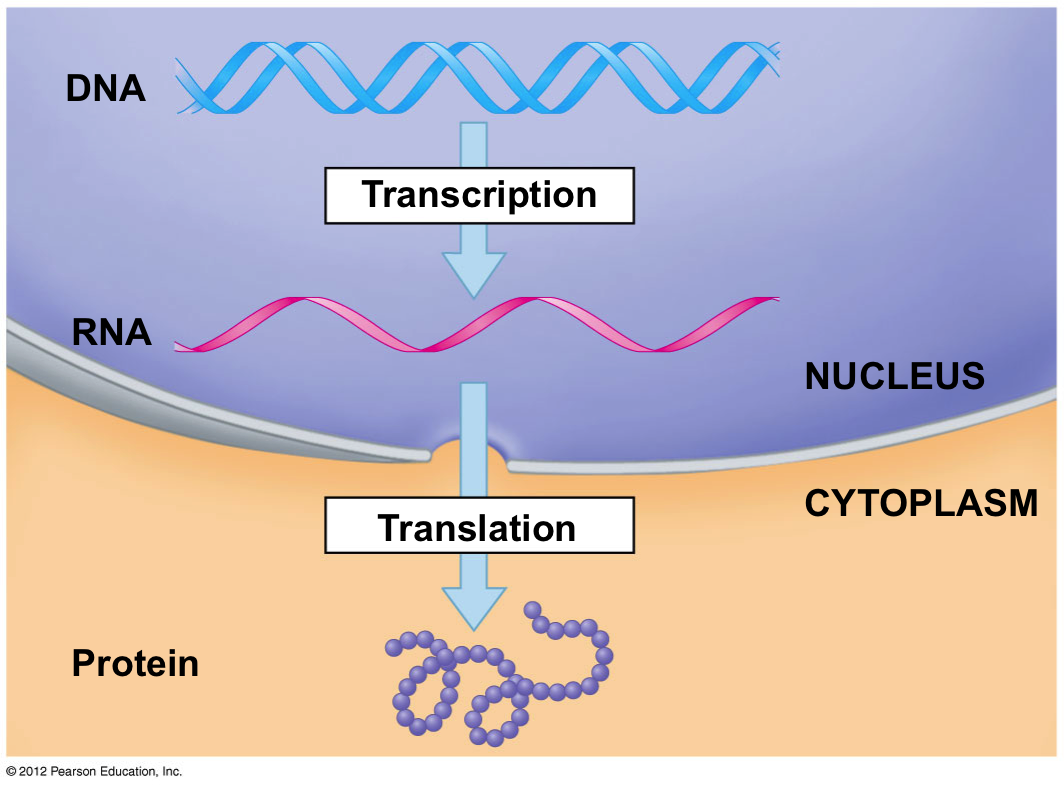
\includegraphics[width=.4\textwidth]{figs/protein.png}
  \uncover<2>{
    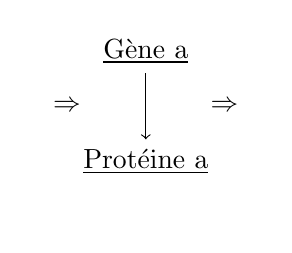
\begin{tikzpicture}
      \path[use as bounding box] (-3, 1) rectangle (0, -1.5);
      \node at (-1.5,.7) (ga) {\underline{Gène a}};
      \node at (-1.5,-0.7) (pa) {\underline{Protéine a}};
      \node[draw=none] at (-2.5,0) {$\Rightarrow$};
      \path[draw,->] (ga) -- (pa);
      \node[draw=none] at (-0.5,0) {$\Rightarrow$};
    \end{tikzpicture}}
  \uncover<2>{
    \scalebox{2}{
    \begin{tikzpicture}[adn]
      \path[use as bounding box] (-.3, .5) rectangle (0.5, -.7);
      \node (a) {a};
    \end{tikzpicture}}
  }
\end{center}

\end{frame}



\begin{frame}[c]
  \frametitle{Discrétisation et asynchronisme}

\begin{center}
  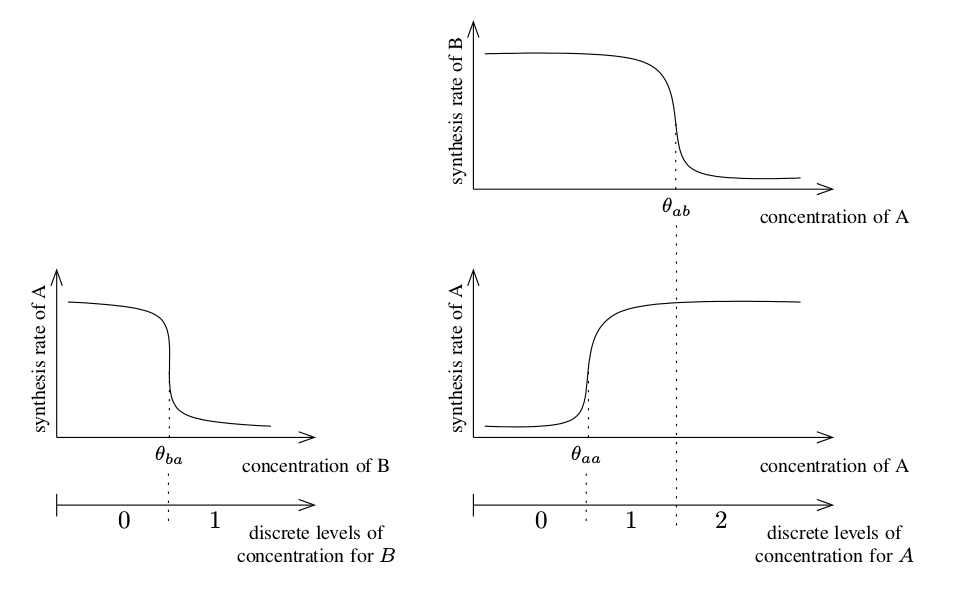
\includegraphics[width=.8\textwidth]{figs/seuils1.png}
\end{center}

\begin{tikzpicture}[adn]
  \path[use as bounding box] (-1.5,-5) rectangle (2.7,-5);
  \node[inner sep=0] (a) at (0,0) {a};
  \node[inner sep=0] (b) at (2,0) {b};
  \path
    node[elabel, below=-1em of a] {$\segm{0}{2}$}
    node[elabel, below=-1em of b] {$\segm{0}{1}$};
  \path
    (a) edge[bend right=15] (b)
    (b) edge[bend right=15] (a)
    (a) edge[loop left] (a);
\end{tikzpicture}

\pause
Concentrations ou niveaux d'activité continus

\quad \f Abstraction sous forme de niveaux discrets correspondant à des seuils

\pause
\medskip
Simultanéité de passage d'un seuil très peu probable

\quad \f Asynchronisme

\end{frame}
